\documentclass{article}
\usepackage{color}
\usepackage{graphicx}
\usepackage{setspace}

\usepackage{geometry}
\usepackage{amsmath}
\usepackage{enumitem,amssymb}
\usepackage{pifont}
\definecolor{darkgreen}{rgb}{0.0, 0.5, 0.0}
\geometry{left = 1.25in, right=1.25in} % New Stuff Learned!
\newcommand{\cmark}{\ding{51}}
\newcommand{\xmark}{\ding{55}}
\newcommand{\done}{\rlap{$\square$}{\raisebox{2pt}{\large\hspace{1pt}\cmark}}
\hspace{-2.5pt}}
\newcommand{\wontfix}{\rlap{$\square$}{\large\hspace{1pt}\xmark}}
\newlist{todolist}{itemize}{2}
\setlist[todolist]{label=$\square$}
\doublespacing
\begin{document}
\begin{titlepage}
\title{\textbf{CHE374 Week 1}}
\author{\textit{Sanzhe Feng}}
\date{\textit{\today}}
\maketitle
\end{titlepage}
\setlength{\parindent}{0pt}

\section*{Cash Flow Diagrams}
\subsection*{Categories of cash flow}
- At the start of a project: \textbf{First(Capital) Cost}: Expense to build/buy and install\\

- During the project: \textbf{Revenues (Sales)}: receipts from sale of products or services; 

\textbf{Operation and Maintenance Costs}: expenses that are incurred on a regular basis (e.g., electricity, labour, repairs)

\textbf{Overhaul}: major (capital) expenditure that occurs part way through the life of an asset\\

- At the end: \textbf{Salvage Value}: net receipt at a project termination for sale/disposal of equipment

\textbf{Scrap value}: value in materials of which item is made

\textbf{Disposal costs}: costs to dispose of waste

\subsection*{Cash-flow Diagrams}
Costs that occur at the start, middle or end of a project is called project life-cycle costs.

A cash-flow diagram is a simple graph that summarises the timing and magituted of cash-flows. X-axis is discrete time periods. Y-axis (implicit): size and direction of cash-flow.
Individual cash-flows are represented by arrows: Down arrow is cash OUTFLOW and UP arrow is CASH inflow.

Unless specified, the end of one period is the beginning of the next. Interest is compounded once per period. Summed cash-flow occurs at the end of the period.
\begin{center}
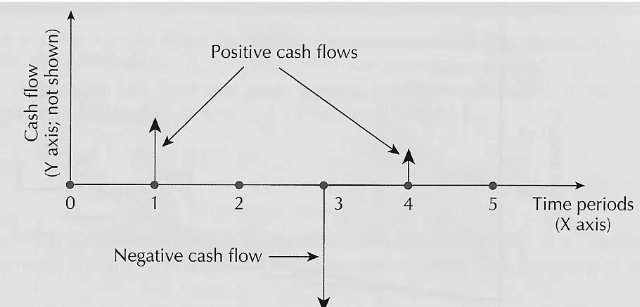
\includegraphics[width=0.5\linewidth]{W2V1.png}
\end{center}

\section*{Cash-flow Categories}

\subsection*{Single payments or receipts}
\begin{center}
    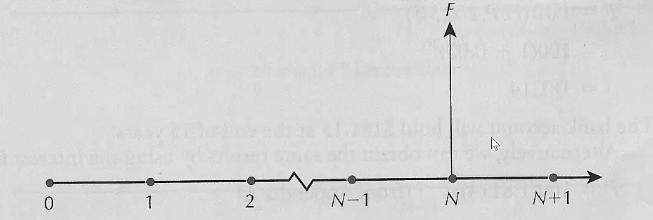
\includegraphics[width=0.5\linewidth]{W2V2_1.png}
\end{center}

\subsection*{Perpetuity}
\begin{center}
    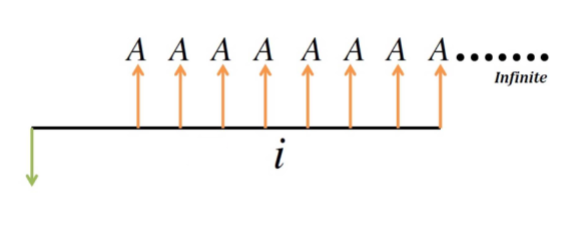
\includegraphics[width=0.5\linewidth]{W2V2_2.png}
\end{center}

\subsection*{Annuity}
\begin{center}
    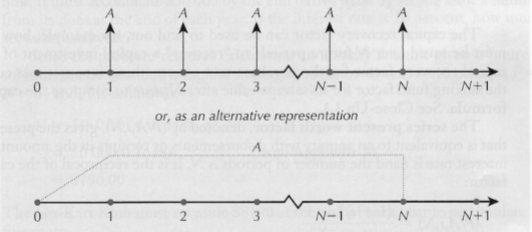
\includegraphics[width=0.5\linewidth]{W2V2_3.png}
\end{center}
\subsection*{Arithmetic gradient}
\begin{center}
    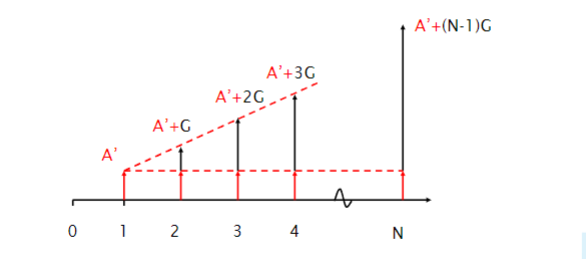
\includegraphics[width=0.5\linewidth]{W2V2_4.png}
\end{center}

\subsection*{Geometric gradient}
\begin{center}
    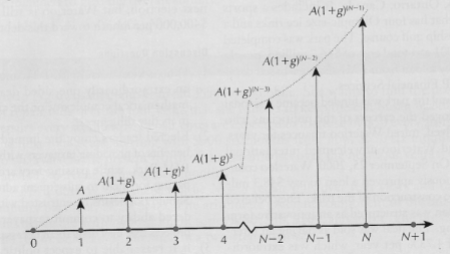
\includegraphics[width=0.5\linewidth]{W2V2_5.png}
\end{center}

\section*{Cash-Flow Equvalence}

\subsection*{Mathematical Equivalence}
A consequence of the mathematical relationship between time and money. For example, two cash-flows $P_t$ and $F_{t+N}$ are mathematically equivalent with respect to interest rate $i$.
\[P_t = \frac{F_{t+N}}{(1+i)^N} \]

\[P_t = \frac{F_{t+N+M}}{(1+i)^{N+M}}\] 

\subsection*{Market Equivalence}
A consequence of the ability to exchange one cash-flow for another at zero cost. 
Exchange future cash=flow for present is borrowing, and the other way around will be lending. 

\subsection*{Decisional Equivalence}
Due to indifference on the part of the decision maker among available choices. 
For a decision maker, two cash-flows, $P_t$ and $F_{t+N}$ are equivalent if he is indifferent between the two. e.g.

Need 1000kg watermelon on 8.15, but offer is 1100kg on 8.23 with same price and payment at the end of August. 
In this case, \textbf{implied} interest rate is 10\% for a week.

\section*{Cash-flow Factors}
\subsection*{Factor Notation}

\[(X/Y, i\%, N)\] reads: X given Y, i, N, where X and Y are chosen from the cash-flow symbols P(Perpetuity), F(Future), A(Annuity) and G(Gradient).
1. $P = F(P/F,i,N)$ This is convert from Future value to present value in year N. For the geometric gradient, we need extra parameter g: $P = G(P/G,i,g,N)$. 

2. Invertbility: $(X/Y,i,N) = 1/(Y/X,i,N)$

3. $(F/P,i,N)$ Compound amount factor $= (1+i)^N$

4. $(P/F,i,N)$ Present worth factor $= (1+i)^{-N}$

5. $(A/F,i,N)$ Sinking fund factor 

6. $(F/A,i,N)$ Series compound amount factor

7. $(A/P,i,N)$ Capital recovery factor 

8. $(P/A,i,N)$ Series present worth factor $= A[\frac{(1+i)^N-1}{i(1+i)^N}]$

9. Present value of a Perpetuity: $A = Pi$

10. Present value of Arithmetic Gradient: Recall previous graph, PV of arithmetic gradient consists of two parts

A. The initial annuity value A that is constant starting at t = 1; $(P/A,i,N)$

B. The growth value G which grows arithmetically starting at t = 2; 
\[ (P/G,i,N) = \frac{1}{i^2}(1-\frac{1+iN}{(1+i)^N})\]
and the overall $P = A(P/A,i,N)+ G(P/G,i,N)$. 

11. Present Value of Geometric Series: as mentioned, for Geometric series, we need the \emph{growth rate}: g;
\[P/G,i,g,N = \frac{1 - (\frac{1+g}{1+i})^N}{i-g} = \frac{(P/A,,i^o,N)}{1+g}\]
where$i^o = \frac{1+i}{1+g} - 1$

12. There is a table that we can use to easily look up for the value of these factors.
\end{document}